\documentclass[tikz]{standalone}
\usetikzlibrary{decorations}
\begin{document}
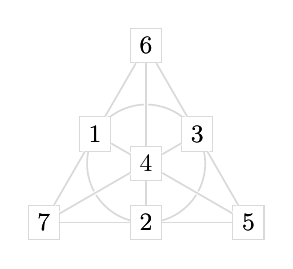
\begin{tikzpicture}[scale=.75]
\tikzset{piping/.style={draw=white,double=gray!30,thin}}
\begin{scope}
\draw[piping] 
(0,0) circle (1);

\foreach \i/\j/\k in {0/5/3,1/6/1,2/7/2}{%
	\node[fill=white,draw=gray!30] at ({2*cos(-30+120*\i)},{2*sin(-30+120*\i)}) {\small\(\j\)};
	\node (\j) at ({2*cos(-30+120*\i)},{2*sin(-30+120*\i)}) {\small\(\j\)};
	\node[fill=white,draw=gray!30] at ({cos(30+120*\i)},{sin(30+120*\i)}) {\small\(\k\)};
	\node (\k) at ({cos(30+120*\i)},{sin(30+120*\i)}) {\small\(\k\)};
}%
\node[fill=white,draw=gray!30] (4) at (0,0) {\small\(4\)};
\draw[piping] (1) -- (4);
\draw[piping] (1) -- (7);
\draw[piping] (2) -- (4);
\draw[piping] (2) -- (5);
\draw[piping] (3) -- (4);
\draw[piping] (3) -- (6);
\draw[piping] (4) -- (5);
\draw[piping] (4) -- (6);
\draw[piping] (4) -- (7);
\draw[piping] (5) -- (3);
\draw[piping] (6) -- (1);
\draw[piping] (7) -- (2);
\end{scope}
\end{tikzpicture}
\end{document}
